\documentclass{beamer}

\setlength{\unitlength}{1cm} 
\usetheme{Frankfurt}
\useoutertheme{infolines}


\usepackage[english]{babel}
\usepackage[utf8]{inputenc}

\usepackage{amsmath, amssymb, mathtools, bbm}
\usepackage{bm}

\usepackage{graphicx}
\usepackage{wrapfig}
\usepackage{tikz} 
\usepackage{relsize}
\usepackage{makecell}
\usepackage{booktabs}
\usepackage{subcaption}
\usepackage{float}
\usepackage{multirow} 

\usepackage[style=apa]{biblatex}
\usepackage{csquotes}

\bibliography{
    ../../../../Desktop/bibliographies/thesis,
    ../maths}


% Graphs
\usetikzlibrary{positioning, arrows.meta, calc, decorations.markings, math, matrix, fit, backgrounds}

\tikzset{fontscale/.style = {font=\relscale{#1}}}

\definecolor{prosumer}{cmyk}{0,0.816,0.408,0}

% Math commands
\newcommand{\E}{\mathbb{E}}
\newcommand{\R}{\mathbb{R}}
\newcommand{\B}{\mathbb{B}}

\newcommand{\matr}[1]{\bm{#1}}
\newcommand{\set}[1]{\left\{#1\right\}}

\newcommand{\Y}{\matr{Y}}
\newcommand{\I}{\matr{I}}
\newcommand{\G}{\matr{G}}
\newcommand{\T}{\matr{T}}

\newcommand{\V}{\mathbb{V}}

% PATHS

\newcommand{\outdiag}{../thesis/sections/diagrams}


\title{How directed is a directed network?}
\author{Andrea Titton}
\title{Thesis defence}
\subtitle{Contagion of Electricity Prices \\ A Dynamic Game of Price Hikes Propagation}
\institute{Tinbergen Institute}
\date{04/12/2020}

\begin{document}

\AtBeginSubsection[]
{
    \begin{frame}
        \frametitle{Table of Contents}
        \tableofcontents[currentsection,currentsubsection]
    \end{frame}
}

\frame{\titlepage}

\begin{frame}
    \tableofcontents
\end{frame}

\section{Introduction}

\begin{frame}{Motivation}
    Green energy transition and advent of \textbf{prosumers}
    \vspace{2em}
    \begin{itemize} \setlength\itemsep{1.5em}
              \pause \item Risk of \textit{local} demand shocks
              \pause \item \textbf{Local quasi-monopolies} energy providers (e.g. ERCOT case in Texas) and decentralized prosumers
              \pause \item Weather shocks lead to \textbf{uncertainty} among risk averse consumers
    \end{itemize}
\end{frame}

\begin{frame}{Lack of price convergence}
    \begin{figure}
        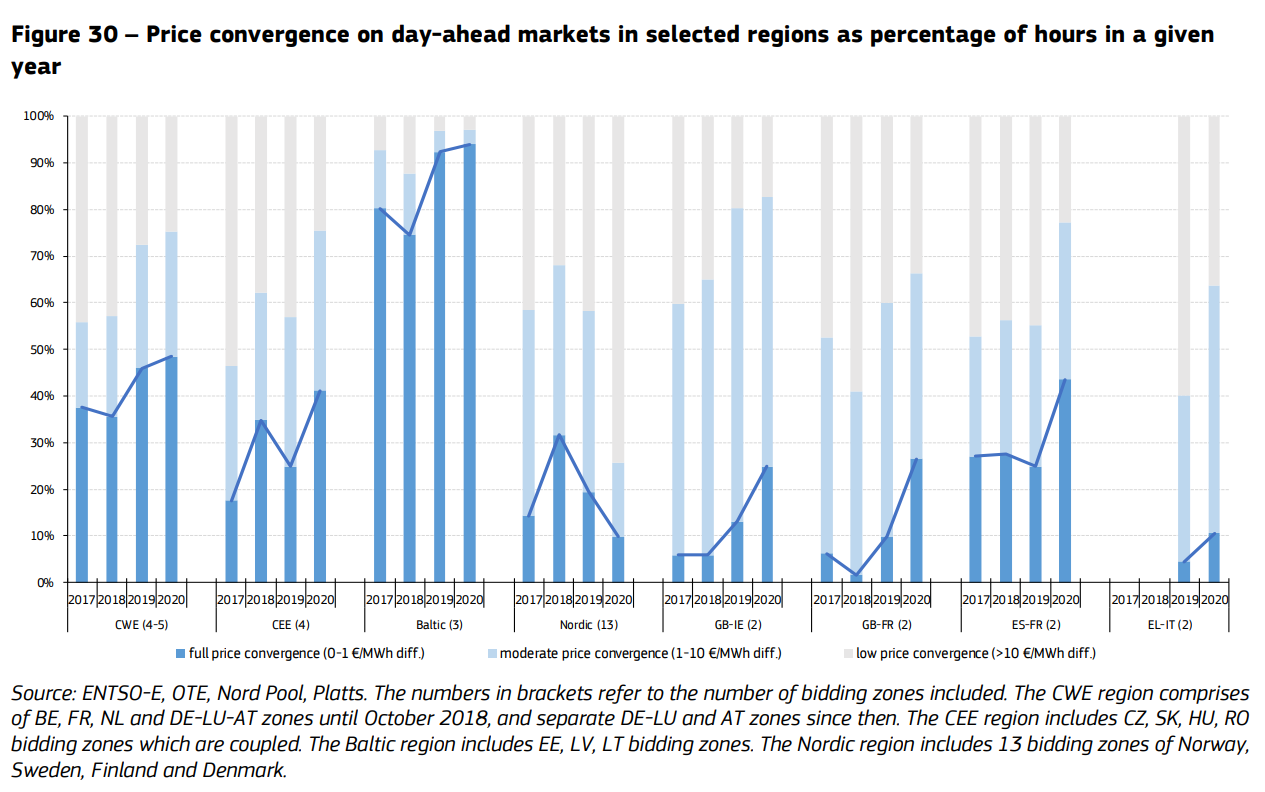
\includegraphics[height = 0.7\textheight]{figures/convergence.PNG}
        \caption{\cite{Report2019}}
    \end{figure}
\end{frame}

\begin{frame}{Research question}

    Prosumers induce three sources of uncertainty: bounded rationality, risk aversion, and renewable energy volatility

    \begin{itemize} \setlength{\itemsep}{1em}
        \item \textit{How do exogenous and unexpected demand shocks affect the price formation mechanism?} \pause
        \item \textit{How do shock in prices transmit to the cross-border market?} \pause
        \item \textit{Hysteresis: can this shock produce sustained price imbalances?} \pause
        \item \textit{Are current policies effective in this framework?}
    \end{itemize}

\end{frame}

\begin{frame}{What is new?}

    Comparison with previous ABM (\cite{Weidlich2008})
    \vfill

    \visible<1->{\begin{minipage}{0.4\textwidth}
            \resizebox{\textwidth}{!}{\tikzstyle{basic} = [
draw,circle,
minimum size=10pt,
]

\tikzstyle{core} = [
draw,circle,
minimum size=10pt,
prosumer,
fill=prosumer,
text=black
]

\begin{tikzpicture}[-{Latex[scale=1]}, thick]

    \node [core] (1) {Consumers};
    \node [core, below = 4cm of 1] (3) {Producers};
    \node [basic, right = 1cm of 1] (2-1) {\makecell[c]{Constant \\ demand}};
    \node [basic, right = 1cm of 3] (4) {\makecell[c]{Market \\ power}};
    \node [basic, above = 1cm of 4] (2-2) {Supply};
    \node [basic, below right = 1cm and 2cm of 2-1] (5) {Prices};


    \path
    (1) edge (2-1)
    (4) edge (2-2)
    (3) edge (4)
    (2-2) edge (5)
    (2-1) edge [dashed, -] (5)
    ;

\end{tikzpicture}}
        \end{minipage}}
    \hfill
    \visible<2->{\begin{minipage}{0.55\textwidth}
            \resizebox{\textwidth}{!}{\tikzstyle{basic} = [
draw,circle,
minimum size=10pt
]

\tikzstyle{core} = [
draw,circle,
minimum size=10pt,
prosumer,
fill=prosumer,
text=black
]


\begin{tikzpicture}[-{Latex[scale=1]}, thick]

    \node [core] (1) {Prosumers};
    \node [core, below = 4cm of 1] (3) {Producers};
    \node [basic, right = 1cm of 1] (2-1) {\makecell[c]{Demand \\ shocks}};
    \node [basic, right = 1cm of 3] (4) {\makecell[c]{Market \\ power}};
    \node [basic, above = 1cm of 4] (2-2) {\makecell[c]{Supply \\ shocks}};
    \node [basic, below right = 1cm and 2cm of 2-1] (5) {Prices};
    \node [basic, right = 1cm of 4] (7) {\makecell[c]{Bargaining \\ power}};
    \node [core, right = 1cm of 7] (6) {Providers};


    \path
    (1) edge (2-1)
    (4) edge (2-2)
    (3) edge (4)
    (2-2) edge (5)
    (2-1) edge (5)
    (6) edge (7)
    (7) edge (4) 
    ;

\end{tikzpicture}}
        \end{minipage}}
\end{frame}

\section{Model}

\begin{frame}{Notation: beliefs $\B$}
    \begin{itemize} \setlength\itemsep{1.5em}
        \item Agents have beliefs over processes $x_t$, denoted by $\B[x_{t+1}]$
        \item These can be dependent on the information available to agents up to time $t$, denoted $\B_t[\cdot]$
    \end{itemize}
\end{frame}

\begin{frame}{Notation: graphs}
    \begin{itemize} \setlength\itemsep{1.5em}
        \item A graph $\mathcal{A}$ is a set of $V$ vertex and $E$, with adjacency matrix $\matr{A}$ \pause
        \item $L(\mathcal{A}) = (V_L, E_L)$ is the associated \textbf{line graph}, with adjacency matrix $\matr{G}$ \pause
        \item $V_L \subseteq V$ and $E_L \subseteq E$ \pause
    \end{itemize}
    \begin{center}
        \resizebox{!}{0.4\textheight}{\tikzstyle{var} = [
draw, dashed,
minimum size=40pt]

\tikzstyle{agent} = [
draw, circle,
minimum size=40pt]

\begin{tikzpicture}[-{Latex[scale=1]}, thick]


    \node [agent] (one) {$1$};
    \node [agent, below = 2cm of one] (five) {$5$};
    \node [agent, left = 2cm of one] (two) {$2$};
    \node [agent, below = 2cm of two] (three) {$3$};
    \node [agent, left = 2cm of three] (four) {$4$};

    
    \path
        (one) edge [above] node {$(1, 2)$} (two)
        (one) edge [left] node {$(1, 4)$} (five)
        (two) edge [right] node {$(2, 3)$} (three)
        (three) edge [below] node {$(3, 4)$} (four);

    \node [var, left = 2cm of two] (A) {$\mathcal{A}$};

    % Second group
    \node [agent, right = 4cm of one] (one-two) {$(1, 2)$};
    \node [agent, below right = 1cm and 1cm of one-two] (one-five) {$(1, 5)$};
    \node [agent, below left = 1cm and 1cm of one-two] (two-three) {$(2, 3)$};
    \node [agent, below = 1cm of two-three] (three-four) {$(3, 4)$};

    \path
        (one-two) edge [above right] node {$1$} (one-five)
        (two-three) edge [above left] node {$2$} (one-two)
        (three-four) edge [left] node {$3$} (two-three);

    \node [var, below = 1cm of one-five] (LA) {$L(\mathcal{A})$};
        

\end{tikzpicture}}
    \end{center}
\end{frame}


\begin{frame}{Model outline}
    \centering
    \only<1>{
        \resizebox{\textwidth}{!}{\tikzstyle{var} = [
draw,circle,
prosumer,
fill=prosumer,
text=black,
minimum size=10pt]

\tikzstyle{agent} = [
draw, circle,
fill=blue!30,
minimum size=10pt]

\tikzstyle{derived} = [
draw, circle, dashed,
minimum size=10pt]

\tikzstyle{time} = [
draw=gray, rectangle,
dashed,
thick,
inner sep=5pt]

\tikzstyle{market} = [
draw=gray, circle,
dashed,
thick,
inner sep=5pt]


\begin{tikzpicture}[-{Latex[scale=1]}, thick, every text node part/.style={align=center, fontscale=0.8}]

    \node [agent] (prov) {Provider};
    \node [market, left = 2cm of prov] (cb-market) {Cross-border \\ market};
    \node [agent, above right = 1cm and 5cm of prov] (prod) {Producers};
    \node [agent, below right = 1cm and 5cm of prov] (pros) {Prosumers};
    \node [market, right = 2cm of prov] (w-market) {Local \\ wholesale \\ market};

    \path
    (cb-market) edge [bend left] node [above] {$Y_t$} (prov)
    (prov) edge [dashed, bend left] node [below] {$P_t$} (cb-market)
    (prov) edge [ bend left] node [above] {$X_t$} (w-market)
    (w-market) edge [dashed, bend left] node [below] {$p_t$} (prov)
    (prod) edge [] node [above left] {$S_t$} (w-market)
    (w-market) edge [{Latex[scale=1]}-{Latex[scale=1]}] node [below left] {$e_t \  M$} (pros)
    ;

\end{tikzpicture}}}
    \only<2>{
        \resizebox{\textwidth}{!}{\tikzstyle{var} = [
draw,circle,
prosumer,
fill=prosumer,
text=black,
minimum size=10pt]

\tikzstyle{agent} = [
draw, circle,
fill=blue!30,
minimum size=10pt]

\tikzstyle{derived} = [
draw, circle, dashed,
minimum size=10pt]

\tikzstyle{time} = [
draw=gray, rectangle,
dashed,
thick,
inner sep=5pt]

\tikzstyle{market} = [
draw=gray, circle,
dashed,
thick,
inner sep=5pt]


\begin{tikzpicture}[-{Latex[scale=1]}, thick, every text node part/.style={align=center, fontscale=0.8}]

    \node [agent] (prov) {Provider};
    \node [market, left = 2cm of prov] (cb-market) {Cross-border \\ market};
    \node [agent, above right = 1cm and 5cm of prov] (prod) {$N$ Producers};
    \node [agent, below right = 1cm and 5cm of prov] (pros) {$M$ Prosumers};
    \node [market, right = 2cm of prov] (w-market) {Local \\ wholesale \\ market};

    \path
    (cb-market) edge [bend left] node [above] (Y) {$Y_t$} (prov)
    (prov) edge [dashed, bend left] node [below] (P) {$P_t$} (cb-market)
    (prov) edge [ bend left] node [above] (X) {$X_t$} (w-market)
    (w-market) edge [dashed, bend left] node [below] (p) {$p_t$} (prov)
    (prod) edge [] node [above left] (S) {$S_t$} (w-market)
    (w-market) edge [{Latex[scale=1]}-{Latex[scale=1]}] node [below left] (e) {$e_t$} (pros)
    ;

    \node[draw, dotted, outer sep = 0, inner sep = 0, fit = (w-market) (e) (p) (X) (S) (prod) (pros)]{};

\end{tikzpicture}}}
\end{frame}

\subsection{Local market}

\begin{frame}{Prosumers}
    \begin{itemize} \setlength\itemsep{1.5em}
        \item M producer pre local market \pause
        \item All with the same ``demand endowment'' $e_t$
    \end{itemize}
\end{frame}

\begin{frame}{Producers setup}
    Main modelling assumption \vspace{5mm}
    \begin{itemize} \setlength\itemsep{1.5em}
        \item Price takers $p_t$ and oligopolist \pause
        \item Produce electricity $s_t$ at fixed marginal cost $k$ \pause
        \item Can ramp-up or down production with a one period delay by $r_t \in [\underline{r}, \overline{r}]$ \pause
        \item $r_t$ costs $c(s_t, r_t) = \max \{0, s_t \ r_t \}$ per unit
    \end{itemize}
\end{frame}


\begin{frame}{Producers optimization}
    \begin{equation*}
        V(s_t, p_t) = \max_{r_t} \left\{ s_t \ \underbrace{(p_t - k)}_{\text{unit profit}} - \underbrace{ c(s_t, r_t) \  r_t }_{\text{ramp-up costs}} + \beta \  V(s_{t+1}, p_{t+1}) \right\}
    \end{equation*}
    \vspace{5mm}
    \visible<2>{\begin{itemize} \setlength\itemsep{1.5em}
            \item $s_{t+1} = s_t + r_t$
            \item Providers are naive: $\B[p_{t+1}] = p_t$
        \end{itemize}}
\end{frame}

\begin{frame}{Marginal costs and benefits}

    The policy function $r(p_t, s_t)$ is such that $mc(r) = mb(r)$.

    \visible<2->{
        \begin{equation*}
            mc = \overbrace{c(s_t, r)}^{\text{cost you pay today}} + \overbrace{r \ \frac{\partial c}{\partial r}(s_t, r)}^{\text{moved to new cost level}}
        \end{equation*}
    }

    \visible<3->{
        \begin{equation*}
            \begin{split}
                \frac{mb}{\beta} &= \overbrace{(p_t - k)}^{\text{unit profit}} + \overbrace{\left(\frac{\partial c}{\partial r}(s_t + r, r) - \frac{\partial c}{\partial s_t}(s_t + r, r)\right)}^{\text{moved to a new level of costs tomorrow}} \ r + \\
                & + \underbrace{c(s_t + r, r)}_{\text{costs you do not pay tomorrow}}
            \end{split}
        \end{equation*}
    }

\end{frame}

\begin{frame}{Policy $r$}
    \visible<1->{
        If equality is possible
        \begin{equation*} \label{rpolicy}
            r(s_t, p_t) =
            \frac{1 - \beta}{\beta} \ s_t - \sqrt{ \left(\frac{1 - \beta}{\beta} \ s_t \right)^2 - \ \left(p_t - k\right) }.
        \end{equation*}

        \begin{itemize}
            \item $r(s_t, p_t) \xrightarrow{} 0$ as $p_t \xrightarrow{} k$
            \item Decreasing in $s_t$ and increasing in $p_t$
        \end{itemize}
    }

    \vfill

    \visible<2->{
        There are two \textit{regions} where equality is not possible:
        \begin{itemize}
            \item If $p_t \leq k$ there are no unit profits, $mc(r) > mb(r)$
            \item If $s_t \leq \frac{\beta}{1-\beta} \sqrt{p_t - k}$ production is too low, $mc(r) < mb(r)$
        \end{itemize}
    }
\end{frame}


\begin{frame}
    \begin{figure}
        \includegraphics[width = 0.8 \textwidth]{../../plots/rfunction.pdf}
    \end{figure}
\end{frame}

\begin{frame}{Demand}
    Let $R_t = \sum^N_{i = 1} r_t$, \\
    then the \textbf{excess demand} in the local market changes as,

    \vspace{0.2\textheight}

    \begin{equation*}
        X_{t+1} - X_t = \underbrace{M \left(e_{t+1} - e_t \right)}_{\text{Increases in demand shocks}} - \underbrace{R_t}_{\text{Decreases in ramp-up}}
    \end{equation*}
\end{frame}

\begin{frame}{Provider local problem}
    \visible<1->{
        The provider $i$ needs to,

        \begin{enumerate}
            \item Pick $p_{t}$ which induces $X_{i, t}$
            \item Trade with its neighbors $N_{\mathcal{A}}(i)$ the quantities $Y^{(i, j)}$ so that $X_{i, t} \leq \sum_j Y^{(i, j)}$
        \end{enumerate}
    }

    \visible<2->{
        \begin{equation*}
            \begin{split}
                V(X_{i, t}, S_{i, t}) = \max_{p_{i, t}, Y^{(i, j)}_t} \Bigg\{ &\overbrace{p_{i, t} \  X_{i, t} - \sum_{j \in N_{\mathcal{A}}(i)} Y^{(i, j)}_t \  P^{(i, j)}(\Y_t)}^{\text{Instantaneous profits}} \\
                &+ \underbrace{\lambda_{i, t} \  \left( X_{i, t} - \sum_{j \in N_{\mathcal{A}}(i)} Y^{(i, j)}_t \right)}_{\text{Constraint}} \\
                &+ \beta \   V(X_{i, t+1}, S_{i, t+1}) \Bigg\}
            \end{split}
        \end{equation*}
    }


\end{frame}


\begin{frame}{Provider's beliefs}

    There are two state variables $X_{i, t}$ and $S_{i, t}$,

    \begin{equation*}
        \begin{split}
            X_{i, t+1} &= X_{i, t} - \B_{i, t} \left[R(p_{i, t}, S_{i, t}) \right] \\
            S_{i, t+1} &= S_{i, t} + \B_{i, t} \left[R(p_{i, t}, S_{i, t}) \right]
        \end{split}
    \end{equation*}

    where,

    \begin{minipage}{.45\textwidth}
        \begin{equation*}
            \begin{split}
                &\B_{i, t} \left[R(p_{i, t}, S_{i, t}) \right] = \\
                &\alpha_{i, t} + \gamma_{i, t} \  p_{i, t} + \eta_{i, t} \ S_{i, t}
            \end{split}
        \end{equation*}
    \end{minipage}
    \hfill
    \begin{minipage}{.45\textwidth}
        \begin{figure}
            \includegraphics[height = 0.4\textheight]{../../plots/constant/star/ols.pdf}
        \end{figure}
    \end{minipage}

\end{frame}

\begin{frame}

    The optimization problem determines the \textbf{local price evolution}
    \begin{equation*}
        p_{i, t+1} = p_{i, t} + \underbrace{\frac{1}{\gamma_{i, t}} \left( \frac{1-\beta}{\beta } X_{i, t} + \alpha_{i, t} + \eta_{i, t} S_{i, t} \right)}_{\text{influence of local market } L_{i, t}(X_{i, t}, S_{i, t})} - \underbrace{\lambda_{i, t}}_{\text{influence of cross-border market}}
    \end{equation*}

\end{frame}

\subsection{Cross-border market}

% CB market
\begin{frame}{Cross-border market}
    \centering
    \resizebox{\textwidth}{!}{\tikzstyle{prosumers} = [
draw,circle,
prosumer,
fill=prosumer,
text=black,
minimum size=5pt]

\tikzstyle{provider} = [
draw,circle,
minimum size=10pt]

\tikzstyle{market} = [
draw=gray, dashed, thick,
inner sep=8pt]


\begin{tikzpicture}[{Latex[scale=0.5]}-{Latex[scale=0.5]}, thick]

    % Placing providers
    \foreach \x/\y [count=\j] in {1/1, -1/1, 1/-1, -1/-1}
        % Draw provider
        {\node [provider]  (\j) at (2*\x, 2*\y) [fontscale=0.8] {\makecell[l]{Prov. \j \\ $X(p_{\j})$}};

            % Draw prosumers
            \edef\points{}
            \foreach \z/\w [count=\i] in {0/2, 1/2.1, 1.75/1.75, 2.1/1, 2/0}
                {\node [prosumers] (\x\y\i) at (\x + 1.3*\x*\z, \y + 1.5*\y*\w) [fontscale=0.6] {$x_{\i}$};
                    \path (\j) edge [] node [fontscale = 0.6] {} (\x\y\i);
                    \xdef\points{(\x\y\i) \points}
                };}

    \path
    (1) edge [-{Latex}] node [above, fontscale=0.8] {$Y^{(1, 2)}$} (2)
    (1) edge [-{Latex}] node [right, fontscale = 0.8] {$Y^{(1, 3)}$} (3)
    (1) edge [-{Latex}] node [above left, fontscale = 0.8] {$Y^{(1, 4)}$} (4)
    (3) edge [-{Latex}] node [above, fontscale = 0.8] {$Y^{(3, 4)}$} (4);

\end{tikzpicture}}
\end{frame}

\begin{frame}{Nash-bargaining}
    Conditional on $\matr{X}_t$ and $\matr{p}_t$ being determined,

    \begin{equation*}
        \begin{split}
            P_t^{(i, j)} &= \arg \max_{P_t^{(i, j)}} \left\{\Pi_{i, t} \  \Pi_{j, t} \right\} \\
            &= \frac{1}{2\  Y_t^{(i, j)}} \times \\
            &\times \left( \underbrace{\Delta^{(i, j)}_t}_{\text{revenue difference }}
            + \underbrace{\sum_{m\in N_{\mathcal{A}}(j)} Y_t^{(j, m)} \  P_t^{(j, m)}}_{\text{outside option of } j}
            - \underbrace{\sum_{m \in N_{\mathcal{A}}(i)} Y_t^{(i, m)} \  P_t^{(i, m)}}_{\text{outside option of } i} \right)
        \end{split}
    \end{equation*}
\end{frame}

\begin{frame}{Back to the first order condition}
    The optimization problem for a neighboring quantity $Y^{(i, m)}$ (suppressing $i$) we obtain,

    \begin{equation*}
        \begin{split}
            -\lambda_t &= \sum_{j \in N_{\mathcal{A}}(i)} \frac{\partial (Y_t^j \  P_t^j(\Y_t))}{\partial Y_t^m} \\
            &= P_t^m(\Y_t) + \sum_{j \in N_{\mathcal{A}}(i) \setminus \set{m}} Y_t^j \  \frac{\partial P_t^j(\Y_t)}{\partial Y_t^m}
        \end{split}
    \end{equation*}
    Using the price just derived we can write $-\lambda_t = 2 P_t^m(\Y_t) $.

\end{frame}

\begin{frame}{Recap}
    \renewcommand{\arraystretch}{3}
    \resizebox{\linewidth}{!}{
        \begin{tabular}{c  c | c }
            Agent            & Actual process                                                                                               & Perceived process                                                                 \\
            \midrule
            \boxed{Provider} & $R_t = \sum^N_{i = 1} r(s_{i, t}, p_t)$                                                                      & $ \B_{t} \left[R_{t+1} \right] = \alpha_{t} + \gamma_{t} \  p_t + \eta_{t} \ S_t$ \\
            \midrule
            \boxed{Producer} & $p_{t+1} = p_t + \frac{1-\beta}{\beta \ \gamma} X_t + \frac{\alpha + \eta S_t}{\gamma} + 2P^m(\matr{Y}_{t})$ & $\B\left[p_{t+1}\right] = p_t$
        \end{tabular}
    }
\end{frame}

\section{Contagion}

\begin{frame}{Bargaining influence matrix}

    Stacking in vectors,

    \begin{equation*}
        \begin{split}
            2(P_t \circ \Y_t) &= \Delta_t  - \G \left( P_t \circ \Y_t \right) \\
            (2\I + \G) (P_t \circ \Y_t) &= \Delta_t  \\
            (P_t \circ \Y_t) &= (2\I + \G)^{-1} \Delta_t
        \end{split}
    \end{equation*}

    Contagion is determined, via $P(\Y_t)$, by

    \begin{equation*}
        (2\I + \G)^{-1}
    \end{equation*}

    called here \textit{bargaining influence matrix}

\end{frame}

\begin{frame}{Star}

    If $\mathcal{A}$ (\textit{left}) is a star graph then $L(\mathcal{A})$ (\textit{right}) is a complete graph. \vspace{5mm}

    \begin{columns}[T,onlytextwidth]

        \begin{column}{.46\textwidth}
            \resizebox{\linewidth}{!}{\tikzstyle{var} = [
draw,circle,
minimum size=10pt]

\tikzstyle{agent} = [
draw, circle,
minimum size=10pt]

\begin{tikzpicture}[-{Latex[scale=1]}, thick]

    \node [agent] (one) {Prov. $1$};
    \node [agent, left = 3cm of one] (two) {Prov. $2$};
    \node [agent, above = 3cm of one] (three) {Prov. $3$};
    \node [agent, right = 3cm of one] (four) {Prov. $4$};


    \path
    (one) edge [] node [above] {$Y^{(1, 2)}$} (two)
    (one) edge [] node [left] {$Y^{(1, 3)}$} (three)
    (one) edge [] node [above] {$Y^{(1, 4)}$} (four);

\end{tikzpicture}}
        \end{column}

        \hfill

        \begin{column}{.46\textwidth}
            \resizebox{\linewidth}{!}{\tikzstyle{var} = [
draw,circle,
minimum size=10pt]

\tikzstyle{agent} = [
draw, circle,
minimum size=10pt]

\begin{tikzpicture}[-, thick]

    \node [agent] (one-two) {$(1, 2)$};
    \node [agent, above right = 1cm and 1cm of one-two] (one-three) {$(1, 3)$};
    \node [agent, below right = 1cm and 1cm of one-three] (one-four) {$(1, 4)$};
    \node [agent, below right = 1cm and 1cm of one-two] (one-n) {$(1, n)$};


    \path
    (one-two) edge [] node {} (one-three)
    (one-two) edge [] node {} (one-four)
    (one-three) edge [] node {} (one-four)
    (one-two) edge [] node {} (one-n)
    (one-three) edge [] node {} (one-n)
    (one-four) edge [] node {} (one-n);

\end{tikzpicture}}
        \end{column}
    \end{columns}
\end{frame}

\begin{frame}{Path}
    If $\mathcal{A}$ (\textit{left}) is a path graph then $L(\mathcal{A})$ (\textit{right}) is a path graph. \vspace{5mm}

    \begin{columns}[T,onlytextwidth]

        \begin{column}{.46\textwidth}
            \resizebox{\linewidth}{!}{\tikzstyle{var} = [
draw,circle,
minimum size=10pt]

\tikzstyle{agent} = [
draw, circle,
minimum size=10pt]

\begin{tikzpicture}[-, thick]

    \node [agent] (one) {Prov. $1$};
    \node [agent, below right = 2cm and 2cm of one] (two) {Prov. $2$};
    \node [agent, below right = 2cm and 2cm of two] (three) {Prov. $3$};
    \node [agent, below right = 2cm and 2cm of three] (four) {Prov. $n$};


    \path
    (one) edge [] node [below left] {$Y^{(1, 2)}$} (two)
    (two) edge [] node [below left] {$Y^{(2, 3)}$} (three)
    (three) edge [dashed] node [below left] {} (four);

\end{tikzpicture}}
        \end{column}

        \hfill

        \begin{column}{.46\textwidth}
            \resizebox{\linewidth}{!}{\tikzstyle{var} = [
draw,circle,
minimum size=10pt]

\tikzstyle{agent} = [
draw, circle,
minimum size=10pt]

\begin{tikzpicture}[-{Latex[scale=1]}, thick]

    \node [agent] (one-two) {$(1, 2)$};
    \node [agent, below right = 2cm and 2cm of one-two] (two-three) {$(2, 3)$};
    \node [agent, below right = 2cm and 2cm of two-three] (three-four) {$(3, 4)$};
    \node [agent, below right = 2cm and 2cm of three-four] (last) {$(n, n-1)$};


    \path
    (one-two) edge [] node [below left] {Prov. $2$} (two-three)
    (two-three) edge [] node [below left] {Prov. $3$} (three-four)
    (three-four) edge [dashed] (last);

\end{tikzpicture}}
        \end{column}
    \end{columns}
\end{frame}

\begin{frame}

    \begin{columns}
        \begin{column}{.46\textwidth}
            \begin{figure}
                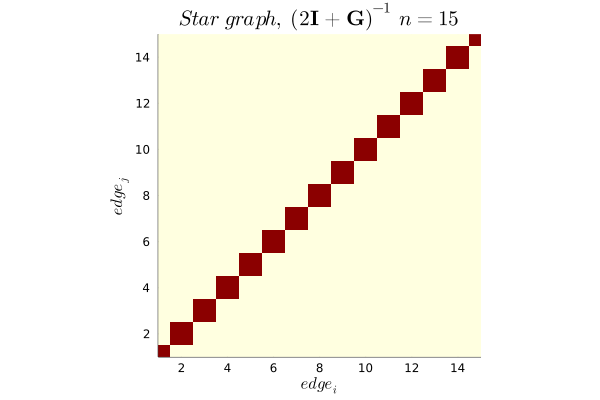
\includegraphics[width = \linewidth]{../../plots/bargmatrices/star.png}
            \end{figure}
        \end{column}

        \hfill

        \begin{column}{.46\textwidth}
            \begin{figure}
                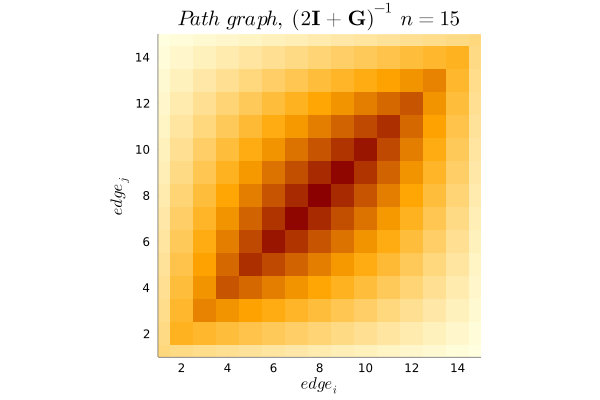
\includegraphics[width = \linewidth]{../../plots/bargmatrices/path.png}
            \end{figure}
        \end{column}
    \end{columns}

    \begin{columns}
        \begin{column}{.46\textwidth}
            \begin{figure}
                \includegraphics[width = \linewidth]{../../plots/pricing.pdf}
            \end{figure}
        \end{column}

        \hfill

        \begin{column}{.46\textwidth}
            \begin{figure}
                \includegraphics[width = \linewidth]{../../plots/pricingpath.pdf}
            \end{figure}
        \end{column}
    \end{columns}
\end{frame}


\iffalse
    \section{Policy}

    \section{Conclusion}
\fi




\begin{frame}[allowframebreaks]{Bibliography}
    \printbibliography
\end{frame}

\end{document}